%initial/final : évolution

Le projet Stibbons a pour but la création d'un langage de programmation multi-agent pour développeurs débutants et avancés, ainsi que d'un environnement de développement l'accompagnant.
La finalité est d'effectuer des simulations de comportements d'agents. Un exemple classique est celui dit \og~des termites~\fg~, qui consiste à modéliser des termites ramassant des brindilles pour former leur termitière.
Pour cela, l'utilisateur définit le comportement d'agents représentant ici les termites, étale des brindilles sur le sol, et observe l'agissement de ses agents faire évoluer le modèle.

\begin{figure}[h]
\centering
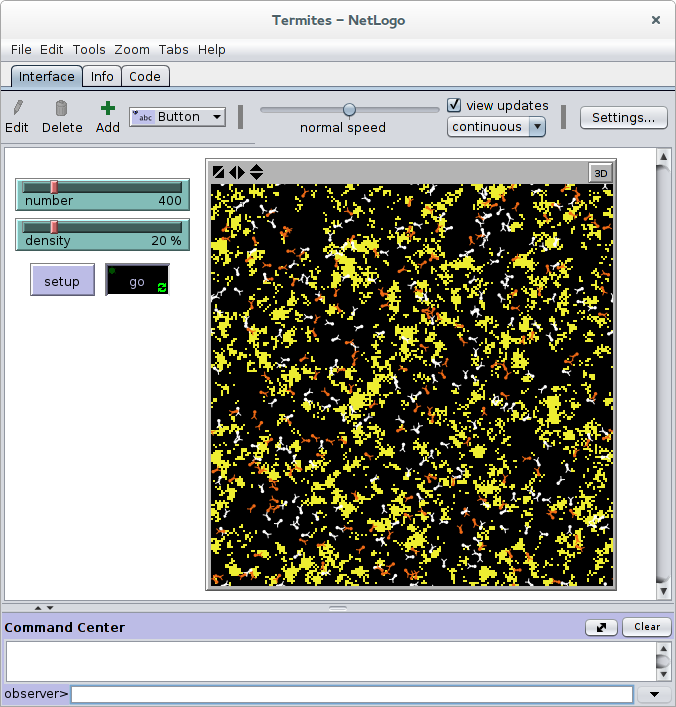
\includegraphics[scale=0.3]{doc/gestionProjet/netlogo-termites.png}
\caption{\label{netlogo-termites} Capture d'écran de NetLogo}
\end{figure}

Notre but initial était d'avoir une application comparable à NetLogo (cf.~\ref{netlogo-code},~\ref{netlogo-termites}), mais exécutant les agents de façon parallèle et non séquencielle comme le fait ce dernier.

\begin{figure}[h]
\centering
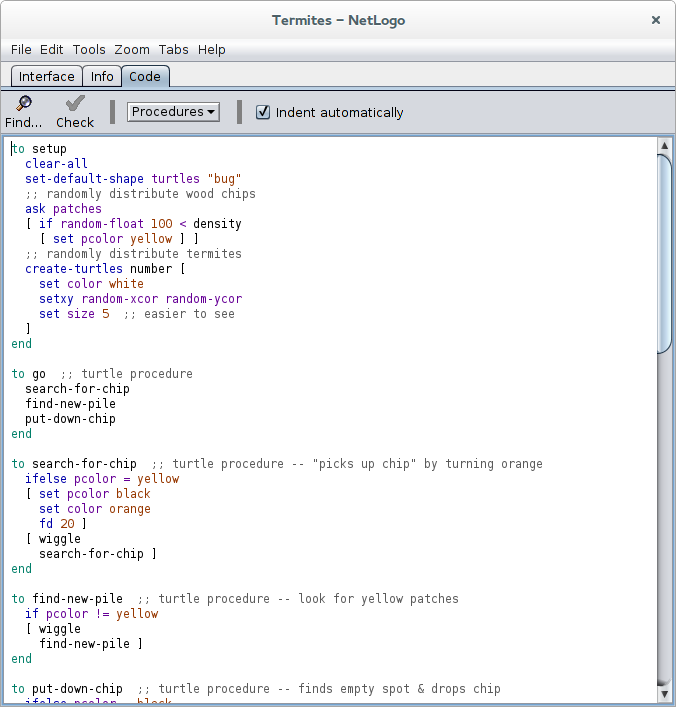
\includegraphics[scale=0.3]{doc/gestionProjet/netlogo-code.png}
\caption{\label{netlogo-code} L'éditeur de texte de NetLogo}
\end{figure}


Nous avons alors décidé de créer un langage permettant de manipuler des agents mobiles (dits tortues) afin de les faire se déplacer et communiquer entre eux, soit directement, soit indirectement en modifiant leur environement. Une interface graphique permettant d'observer directement l'évolution du modèle était également prévue.

Au cours du projet, notre tuteur, Michel Meynard, nous a suggéré de rajouter l'exportation du modèle en cours d'exécution (comprenant l'état du monde, des zones le constituant, et des tortues y évoluant), que nous avons donc rajouté à notre backlog, et à terme à notre application.
Plus tard, nous avons aussi imaginé un programme complémentaire à notre application, qui serait utilisable en ligne de commande et ne nécessiterait pas l'utilisation d'un serveur graphique pour fonctionner, mais permettant d'exporter le modèle à intervalle régulier.
Cela permet, lorsqu'on fait une simulation longue de ne pas utiliser les ressources graphiques de l'ordinateur. En outre, cela permet d'exécuter la simulation à pleine vitesse.
Nous avons également décidé d'intégrer un éditeur de texte à l'application principale afin de pouvoir directement éditer et exécuter un programme Stibbons.
